\documentclass[conference]{IEEEtran}

% ── Paquetes ────────────────────────────────────────────────
\usepackage[utf8]{inputenc}
\usepackage{amsmath, amssymb, amsthm}
\usepackage{graphicx}
\usepackage{float}
\usepackage{cite}
\usepackage{url}
\usepackage{hyperref}
\usepackage{booktabs}
\usepackage{array}
\usepackage{listings}
\usepackage{xcolor}
\usepackage{mathtools}
\usepackage{multirow}
\usepackage{subcaption}

\graphicspath{{imagenes/}}

% Configuración listings Python
\lstset{
  language=Python,
  basicstyle=\ttfamily\scriptsize,
  keywordstyle=\color{blue}\bfseries,
  commentstyle=\color{gray!70}\itshape,
  stringstyle=\color{orange!80!black},
  breaklines=true,
  frame=single,
  rulecolor=\color{gray!40},
  numbers=left,
  numberstyle=\tiny\color{gray},
  captionpos=b,
  showstringspaces=false,
  tabsize=4
}

% Entornos matemáticos
\newtheorem{teorema}{Teorema}
\newtheorem{definicion}{Definición}
\newtheorem{corolario}{Corolario}
\newtheorem{lema}{Lema}
\newtheorem{proposicion}{Proposición}
\newtheorem{observacion}{Observación}

% ── Portada ─────────────────────────────────────────────────
\title{Procesamiento Digital de Imágenes mediante la\\
       Transformada Rápida de Fourier en 2D:\\
       Filtrado Gaussiano Paso-Bajo, Análisis Espectral\\
       y Evaluación Cuantitativa}

\author{
  \IEEEauthorblockN{Integrante 1\IEEEauthorrefmark{1},
                    Integrante 2\IEEEauthorrefmark{1},
                    Integrante 3\IEEEauthorrefmark{1},
                    Integrante 4\IEEEauthorrefmark{1},
                    Integrante 5\IEEEauthorrefmark{1}}
  \IEEEauthorblockA{\IEEEauthorrefmark{1}Departamento de Matemática,
    Facultad de Ingeniería y Arquitectura\\
    Universidad Centroamericana ``José Simeón Cañas''\\
    Antiguo Cuscatlán, El Salvador\\
    Análisis Numérico --- Ciclo 01-2026\\
    Ing. Daniel Augusto Sosa \quad Instructor: Pablo Vides}
}

\begin{document}
\maketitle

% ── Abstract ────────────────────────────────────────────────
\begin{abstract}
Este trabajo presenta un estudio teórico-experimental exhaustivo de la
Transformada Discreta de Fourier en dos dimensiones (DFT-2D) y su
implementación eficiente mediante el algoritmo de Cooley-Tukey (FFT-2D),
aplicadas al procesamiento digital de imágenes RGB. Se desarrolla un flujo
computacional completo que comprende la carga y redimensionado proporcional
de imágenes, el análisis espectral por canal, la modelación del ruido blanco
gaussiano aditivo, el diseño e implementación de un filtro gaussiano paso-bajo
en el dominio de la frecuencia, la reconstrucción mediante IFFT-2D, y la
evaluación cuantitativa mediante el Error Cuadrático Medio (MSE) y el
índice de calidad PSNR. El marco teórico incluye demostraciones de los
teoremas de convolución, Parseval y separabilidad, junto con el análisis
de complejidad computacional del algoritmo FFT. Los experimentos varían el
parámetro $\sigma \in \{10, 30, 60, 200\}$ del filtro gaussiano y muestran
cuantitativamente el compromiso entre supresión de ruido y preservación
de detalle. Se incluye evidencia visual del proceso completo mediante
comparaciones imagen original / imagen con ruido / imagen filtrada para
distintos valores de $\sigma$.
\end{abstract}

\begin{IEEEkeywords}
DFT 2D, FFT, filtro gaussiano paso-bajo, procesamiento de imágenes,
ruido gaussiano, MSE, PSNR, Teorema de Convolución, Cooley-Tukey, NumPy.
\end{IEEEkeywords}

%=============================================================
\section{Introducción}
%=============================================================

El procesamiento digital de imágenes es una de las disciplinas de mayor
impacto tecnológico en la actualidad. Sus aplicaciones abarcan la medicina
(tomografías, resonancias magnéticas, histología digital), la astronomía
(procesamiento de imágenes del telescopio James Webb), las comunicaciones
(compresión JPEG y MPEG), la visión computacional (detección de objetos,
reconocimiento facial) y la seguridad (análisis forense de imágenes,
esteganografía) \cite{gonzalez2018}. En todos estos dominios, el análisis
en el espacio de frecuencias proporciona herramientas que son imposibles o
prohibitivamente costosas de implementar directamente en el dominio espacial.

La idea de descomponer una señal en sus componentes frecuenciales fue
introducida por Jean-Baptiste Joseph Fourier en 1807 para el análisis
del calor, pero su impacto se extendió rápidamente a prácticamente todas
las ramas de la física y la ingeniería. Para imágenes digitales, la
Transformada Discreta de Fourier (DFT) ofrece una representación dual que
revela la distribución de energía en frecuencias espaciales: los coeficientes
de baja frecuencia capturan la estructura global (iluminación, gradientes
suaves), mientras que los de alta frecuencia representan los detalles finos
(bordes, texturas, ruido) \cite{oppenheim1999}.

Sin embargo, la evaluación directa de la DFT-2D tiene una complejidad
computacional de $\mathcal{O}(M^2N^2)$ para una imagen de $M\times N$
píxeles, lo que la hace impráctica para imágenes modernas. El algoritmo de
la Transformada Rápida de Fourier (FFT), cuya versión más difundida fue
publicada por Cooley y Tukey en 1965 \cite{cooley1967}, reduce esta
complejidad a $\mathcal{O}(MN\log MN)$ explotando la estructura recursiva
y separable de la DFT. Esta reducción es la que hace viable el procesamiento
de imágenes en tiempo real.

El filtrado gaussiano paso-bajo en el dominio de la frecuencia es una
de las operaciones más estudiadas en procesamiento de imágenes. A diferencia
del filtro rectangular ideal, el gaussiano no introduce el fenómeno de
\textit{ringing} (oscilaciones de Gibbs) en la imagen reconstruida, gracias
a que su respuesta al impulso es también una función gaussiana (la gaussiana
es la única función que es su propia transformada de Fourier, salvo escala)
\cite{gonzalez2018}. Esto lo convierte en la opción preferida cuando se
requiere suavizado con mínima distorsión de bordes.

Este documento se estructura como sigue: la Sección~\ref{sec:antecedentes}
sitúa el trabajo en el contexto histórico y de literatura relacionada. La
Sección~\ref{sec:marco} desarrolla el marco teórico completo. La
Sección~\ref{sec:filtros_adicionales} presenta otros tipos de filtros
frecuenciales relevantes. La Sección~\ref{sec:metricas} detalla las métricas
de calidad utilizadas. La Sección~\ref{sec:metodologia} describe la
metodología. La Sección~\ref{sec:resultados} presenta los resultados con
evidencia visual y análisis cuantitativo. Finalmente,
la Sección~\ref{sec:conclusiones} presenta conclusiones y limitantes.

%=============================================================
\section{Antecedentes y Contexto}
\label{sec:antecedentes}
%=============================================================

\subsection{Historia del Análisis de Fourier en Imágenes}

El procesamiento de imágenes en el dominio de la frecuencia tiene sus raíces
en la óptica de Fourier del siglo XIX. La primera aplicación sistemática de
la transformada de Fourier al procesamiento digital de imágenes se atribuye
al trabajo de Cooley y Tukey \cite{cooley1967}, que hizo computacionalmente
factible el análisis espectral. En la década de 1970, el estándar JPEG adoptó
la Transformada Discreta del Coseno (DCT), variante de la DFT, como base de
la compresión de imágenes, consolidando el papel central de las técnicas
frecuenciales en la ingeniería multimedia \cite{gonzalez2018}.

\subsection{El Ruido en Imágenes Digitales}

El ruido en imágenes digitales puede tener múltiples orígenes: ruido
térmico del sensor (modelado como gaussiano), ruido de disparo o \textit{shot
noise} (modelado como Poisson), ruido impulsivo o de sal y pimienta, y
artefactos de cuantización. El modelo de ruido blanco gaussiano aditivo
(AWGN) es el más extendido en la literatura por su tratabilidad matemática
y porque representa adecuadamente el ruido térmico de los sensores CCD y
CMOS \cite{oppenheim1999}.

La característica definidora del ruido blanco es que su densidad espectral
de potencia (PSD) es constante para todas las frecuencias:
\begin{equation}
  S_{\eta\eta}(u,v) = \sigma_\eta^2, \quad \forall\,(u,v)
  \label{eq:psd_ruido}
\end{equation}
Esto implica que en el espectro de la imagen ruidosa, el ruido contribuye
homogéneamente a todas las frecuencias, elevando el piso espectral. Los
filtros paso-bajo atenúan las frecuencias altas donde la relación
señal-ruido es más baja, reduciendo la potencia del ruido al costo de
sacrificar algunos detalles finos.

\subsection{Estado del Arte en Filtrado de Imágenes}

Más allá del filtrado gaussiano clásico, el estado del arte incluye:
el filtro de Wiener \cite{oppenheim1999}, que minimiza el MSE asumiendo
estadísticas conocidas de señal y ruido; los métodos de umbralización
wavelet (Donoho y Johnstone, 1994); los filtros bilaterales que preservan
bordes; y más recientemente, las redes neuronales convolucionales profundas
(DnCNN, FFDNet) que aprenden el mapeo ruido$\to$imagen limpia
\cite{gonzalez2018}. El filtrado gaussiano en el dominio de Fourier que
se estudia aquí representa el punto de partida histórico y teórico de todos
estos desarrollos.

%=============================================================
\section{Marco Teórico}
\label{sec:marco}
%=============================================================

\subsection{Representación Discreta de Imágenes Digitales}

Una imagen digital en escala de grises se modela como una función discreta
de dos variables enteras:
\begin{equation}
  f:\{0,\ldots,M{-}1\}\times\{0,\ldots,N{-}1\}\longrightarrow\{0,\ldots,255\}
  \label{eq:img_gray}
\end{equation}
donde $f[m,n]$ representa la intensidad luminosa (nivel de gris) en el
píxel de la fila $m$ y la columna $n$. El conjunto de valores $\{0,\ldots,255\}$
corresponde a la cuantización de 8 bits por canal, estándar en imágenes
digitales comunes.

Para imágenes a color en el espacio RGB, la imagen se representa como un
tensor tridimensional:
\begin{equation}
  \mathbf{f}[m,n] = \bigl(f_R[m,n],\; f_G[m,n],\; f_B[m,n]\bigr) \in \mathbb{R}^3
  \label{eq:img_rgb}
\end{equation}
Esta separación en canales es la clave del procesamiento implementado: al
tratar cada canal como una imagen de escala de grises independiente, se
pueden aplicar todas las herramientas de la DFT-2D de forma directa,
canal por canal.

\subsection{La Transformada Discreta de Fourier en 2D}

\begin{definicion}[DFT 2D]
  Para una imagen discreta $f[m,n]$ de tamaño $M\times N$, la
  \textbf{Transformada Discreta de Fourier en 2D} es la transformación
  lineal $\mathcal{F}: \mathbb{C}^{M\times N}\to\mathbb{C}^{M\times N}$
  definida por:
  \begin{equation}
    F[u,v] = \sum_{m=0}^{M-1}\sum_{n=0}^{N-1}
             f[m,n]\,e^{-j2\pi\!\left(\frac{um}{M}+\frac{vn}{N}\right)}
    \label{eq:dft2d}
  \end{equation}
  con $u\in\{0,\ldots,M{-}1\}$ y $v\in\{0,\ldots,N{-}1\}$.
\end{definicion}

Introduciendo el \textit{twiddle factor} $W_M = e^{-j2\pi/M}$, la DFT-2D
se escribe compactamente como:
\begin{equation}
  F[u,v] = \sum_{m=0}^{M-1}\sum_{n=0}^{N-1}
           f[m,n]\,W_M^{um}\,W_N^{vn}
  \label{eq:dft2d_twiddle}
\end{equation}

Cada coeficiente $F[u,v]\in\mathbb{C}$ encapsula dos tipos de información:
\begin{itemize}
  \item \textbf{Magnitud} $|F[u,v]|$: cuantifica la energía de la componente
    sinusoidal de frecuencias $(u/M,\,v/N)$ ciclos/píxel.
  \item \textbf{Fase} $\angle F[u,v] = \arctan\!\bigl(\mathrm{Im}/\mathrm{Re}\bigr)$:
    codifica el desplazamiento espacial de esa componente.
\end{itemize}

\begin{observacion}
  El componente $F[0,0]$ es la \textbf{componente de continua} (DC) y
  vale $\sum_{m,n} f[m,n]$, es decir, la suma total de intensidades de la
  imagen. Es el coeficiente de mayor magnitud en imágenes naturales.
\end{observacion}

\subsection{Transformada Discreta Inversa (IDFT 2D)}

\begin{definicion}[IDFT 2D]
  Dado el espectro $F[u,v]$, la imagen original se recupera exactamente
  mediante la transformada inversa:
  \begin{equation}
    f[m,n] = \frac{1}{MN}\sum_{u=0}^{M-1}\sum_{v=0}^{N-1}
             F[u,v]\,e^{j2\pi\!\left(\frac{um}{M}+\frac{vn}{N}\right)}
    \label{eq:idft2d}
  \end{equation}
\end{definicion}

La pareja DFT/IDFT constituye una \textit{transformación biyectiva}: no
se pierde información al transformar al dominio de la frecuencia y volver
al dominio espacial. La pérdida de información en el filtrado ocurre
exclusivamente al multiplicar por la función de transferencia $H[u,v]$,
que suprime ciertos coeficientes.

\subsection{Centrado del Espectro: \texttt{fftshift}}

Por convención computacional, la FFT coloca el coeficiente DC en la
posición $(0,0)$ (esquina superior izquierda). La operación \texttt{fftshift}
reubica el DC al centro de la matriz mediante una traslación circular:
\begin{equation}
  F_{\text{shift}}[u,v] = F\!\left[\left(u+\tfrac{M}{2}\right)\!\bmod M,\;
                           \left(v+\tfrac{N}{2}\right)\!\bmod N\right]
  \label{eq:fftshift}
\end{equation}

Esta traslación circular no modifica magnitudes ni fases; es puramente
una reordenación del arreglo que facilita la visualización del espectro
y la construcción de filtros de simetría radial centrados en el DC.

\subsection{Visualización del Espectro: Escala Logarítmica}

El rango dinámico del espectro de magnitud es típicamente de varios
órdenes de magnitud. Para visualizarlo se aplica la compresión logarítmica:
\begin{equation}
  S_c[u,v] = \log\!\bigl(|F_{\text{shift},c}[u,v]| + 1\bigr)
  \label{eq:log_spectrum}
\end{equation}
La constante $+1$ evita singularidades logarítmicas cuando $|F|=0$ y
desplaza el rango para incluir el cero como valor visualizable. La escala
logarítmica comprime el rango dinámico haciendo visibles tanto el pico DC
como los coeficientes de menor energía en las frecuencias altas.

\subsection{Propiedades Algebraicas de la DFT-2D}

La DFT-2D satisface un conjunto de propiedades que son la base teórica
del filtrado espectral \cite{oppenheim1999, gonzalez2018}:

\begin{teorema}[Linealidad]
  Para $\alpha, \beta \in \mathbb{C}$ y $f[m,n]$, $g[m,n]$:
  \begin{equation}
    \mathcal{F}\{\alpha f + \beta g\} = \alpha F[u,v] + \beta G[u,v]
    \label{eq:linealidad}
  \end{equation}
\end{teorema}

\begin{teorema}[Desplazamiento Espacial]
  Un desplazamiento circular $(m_0, n_0)$ en el dominio espacial
  introduce un cambio de fase lineal en el dominio frecuencial:
  \begin{equation}
    f[m{-}m_0, n{-}n_0] \xleftrightarrow{\;\mathcal{F}\;}
    F[u,v]\,e^{-j2\pi\!\left(\frac{um_0}{M}+\frac{vn_0}{N}\right)}
    \label{eq:desplazamiento}
  \end{equation}
  Las magnitudes espectrales no cambian; solo las fases. Esto implica que
  la posición de los objetos en la imagen afecta la fase pero no el espectro
  de potencia.
\end{teorema}

\begin{teorema}[Convolución Circular en 2D]
  \label{teo:conv}
  La convolución circular bidimensional de $f[m,n]$ con $h[m,n]$
  corresponde a la multiplicación punto a punto de sus espectros:
  \begin{equation}
    (f \circledast h)[m,n]
    \;\xleftrightarrow{\;\mathcal{F}\;}\;
    F[u,v]\cdot H[u,v]
    \label{eq:conv_theorem}
  \end{equation}
  \begin{proof}[Demostración (esquema)]
    Por definición de la convolución circular $y[m,n] = \sum_{k,l} f[k,l]\,h[m{-}k,n{-}l]$,
    aplicando la DFT:
    \begin{align*}
      Y[u,v] &= \sum_{m,n} y[m,n]\,W_M^{um}W_N^{vn} \\
             &= \sum_{m,n}\sum_{k,l} f[k,l]\,h[m{-}k,n{-}l]\,W_M^{um}W_N^{vn}
    \end{align*}
    Sustituyendo $m'=m{-}k$, $n'=n{-}l$ y usando la periodicidad de
    $W_M^{u(m'+k)} = W_M^{um'}W_M^{uk}$:
    \begin{align*}
      Y[u,v] &= \left(\sum_{k,l}f[k,l]W_M^{uk}W_N^{vl}\right)
               \left(\sum_{m',n'}h[m',n']W_M^{um'}W_N^{vn'}\right) \\
             &= F[u,v]\cdot H[u,v] \qquad \square
    \end{align*}
  \end{proof}
\end{teorema}

Este teorema es el fundamento del filtrado espectral: en lugar de convolucionar
$f$ con la respuesta impulsional $h$ del filtro (operación de costo
$\mathcal{O}(M^2N^2)$), se multiplican sus espectros (costo $\mathcal{O}(MN)$
más el costo de las FFT).

\begin{teorema}[Parseval en 2D]
  \label{teo:parseval}
  La energía total de la imagen se conserva bajo la DFT-2D:
  \begin{equation}
    \sum_{m=0}^{M-1}\sum_{n=0}^{N-1}|f[m,n]|^2
    = \frac{1}{MN}\sum_{u=0}^{M-1}\sum_{v=0}^{N-1}|F[u,v]|^2
    \label{eq:parseval2d}
  \end{equation}
  \begin{proof}
    Usando la definición de la IDFT~\eqref{eq:idft2d} y desarrollando el
    producto interno:
    \begin{align*}
      \sum_{m,n}|f[m,n]|^2 &= \sum_{m,n} f[m,n]\,\overline{f[m,n]} \\
      &= \sum_{m,n} f[m,n]\,\overline{\frac{1}{MN}\sum_{u,v}F[u,v]W_M^{-um}W_N^{-vn}} \\
      &= \frac{1}{MN}\sum_{u,v}F[u,v]\sum_{m,n}\overline{f[m,n]}W_M^{um}W_N^{vn}
    \end{align*}
    Reconociendo que $\sum_{m,n}\overline{f[m,n]}W_M^{um}W_N^{vn} = \overline{F[u,v]}$
    (por la simetría conjugada de la DFT para señales reales):
    \begin{equation*}
      \sum_{m,n}|f[m,n]|^2 = \frac{1}{MN}\sum_{u,v}|F[u,v]|^2 \qquad \square
    \end{equation*}
  \end{proof}
\end{teorema}

\begin{corolario}
  La energía eliminada por el filtro espectral $H[u,v]$ es exactamente:
  \begin{equation}
    E_{\text{eliminada}} = \frac{1}{MN}\sum_{u,v}|F[u,v]|^2\,(1-H[u,v]^2)
    \label{eq:energia_eliminada}
  \end{equation}
  lo que permite calcular a priori el impacto energético del filtrado
  sin necesidad de ejecutar la IFFT.
\end{corolario}

\begin{teorema}[Separabilidad de la DFT-2D]
  \label{teo:sep}
  La DFT-2D puede calcularse como la composición de DFT-1D aplicadas
  sucesivamente a las filas y luego a las columnas:
  \begin{equation}
    F[u,v] = \sum_{m=0}^{M-1}W_M^{um}
             \underbrace{\left[\sum_{n=0}^{N-1}f[m,n]W_N^{vn}\right]}_{G[m,v]}
    \label{eq:separabilidad}
  \end{equation}
  donde $G[m,v]$ es la DFT-1D de la $m$-ésima fila.
\end{teorema}

Esta separabilidad es la clave algorítmica: aplicar $M$ DFT-1D de longitud $N$
(para las filas) y luego $N$ DFT-1D de longitud $M$ (para las columnas) tiene
costo total $\mathcal{O}(MN\log MN)$ usando el algoritmo FFT-1D.

\begin{proposicion}[Simetría Conjugada]
  Para imágenes reales $f[m,n]\in\mathbb{R}$:
  \begin{equation}
    F[M{-}u,\,N{-}v] = F^*[u,v]
    \label{eq:simetria}
  \end{equation}
  En consecuencia, el espectro de una imagen real es hermitiano: la
  mitad de los coeficientes es la conjugada de la otra mitad, y el
  espectro de magnitud es simétrico respecto al centro.
\end{proposicion}

\subsection{El Algoritmo FFT de Cooley-Tukey}

El algoritmo Cooley-Tukey \cite{cooley1967} aplica el paradigma
\textit{divide y conquista} a la DFT-1D de longitud $N$ (potencia de 2).
Separa la secuencia en muestras pares e impares:
\begin{equation}
  X[k] = \underbrace{\sum_{n=0}^{N/2-1}x[2n]W_{N/2}^{kn}}_{E[k]}
          + W_N^k\underbrace{\sum_{n=0}^{N/2-1}x[2n+1]W_{N/2}^{kn}}_{O[k]}
  \label{eq:fft_decimacion}
\end{equation}

Usando la periodicidad $E[k+N/2]=E[k]$ y $O[k+N/2]=O[k]$:
\begin{align}
  X[k]       &= E[k] + W_N^k\cdot O[k], \quad k=0,\ldots,N/2{-}1
  \label{eq:butterfly_a}\\
  X[k+N/2]   &= E[k] - W_N^k\cdot O[k]
  \label{eq:butterfly_b}
\end{align}

Estas dos ecuaciones definen la \textbf{operación mariposa} (\textit{butterfly}).
Aplicando la recursión $\log_2 N$ veces se reduce el número de multiplicaciones
complejas de $N^2$ a $\frac{N}{2}\log_2 N$. La Tabla~\ref{tab:complejidad}
muestra la reducción de costo para tamaños típicos.

\begin{table}[H]
  \centering
  \caption{Multiplicaciones complejas: DFT directa vs.\ FFT}
  \label{tab:complejidad}
  \begin{tabular}{crrc}
    \toprule
    \textbf{Tamaño} & \textbf{DFT directa} & \textbf{FFT} & \textbf{Factor} \\
    \midrule
    $128\!\times\!128$ & $2.68\times10^8$    & $2.80\times10^5$ & $\sim\!960\times$      \\
    $256\!\times\!256$ & $4.29\times10^9$    & $1.31\times10^6$ & $\sim\!3{,}280\times$  \\
    $512\!\times\!512$ & $6.87\times10^{10}$ & $6.03\times10^6$ & $\sim\!11{,}400\times$ \\
    $1024\!\times\!1024$ & $1.10\times10^{12}$ & $2.75\times10^7$ & $\sim\!40{,}000\times$ \\
    \bottomrule
  \end{tabular}
\end{table}

\subsection{Modelo de Ruido Gaussiano Blanco Aditivo}

El ruido blanco gaussiano aditivo (AWGN) en cada canal RGB se modela como:
\begin{equation}
  \eta_c[m,n] \overset{\text{i.i.d.}}{\sim} \mathcal{N}(0,\,\sigma_\eta^2),
  \quad c\in\{R,G,B\}
  \label{eq:ruido}
\end{equation}

La imagen degradada resultante es:
\begin{equation}
  f_{\text{ruido}}[m,n,c]
  = \mathrm{clip}\bigl(f[m,n,c] + \eta_c[m,n],\; 0,\; 255\bigr)
  \label{eq:imagen_ruidosa}
\end{equation}

La densidad espectral de potencia (PSD) del ruido blanco es constante:
$S_{\eta\eta}(u,v) = \sigma_\eta^2$ para todo $(u,v)$. Esto significa que
en el espectro de Fourier el ruido aporta igual energía a todas las
frecuencias, elevando uniformemente el piso espectral. El filtro paso-bajo
elimina la contribución del ruido en las frecuencias altas al costo de
atenuar también los detalles de alta frecuencia de la imagen original.

\subsection{El Filtro Gaussiano Paso-Bajo}

\begin{definicion}[Filtro Gaussiano Paso-Bajo]
  La función de transferencia del filtro gaussiano paso-bajo centrada en
  $(u_0,v_0)=(M/2,N/2)$ es:
  \begin{equation}
    H[u,v] = \exp\!\left(-\frac{(u-u_0)^2+(v-v_0)^2}{2\sigma^2}\right)
    \label{eq:filtro_gaussiano}
  \end{equation}
  donde $\sigma>0$ es el \emph{parámetro de ancho de banda}.
\end{definicion}

El filtro satisface:
\begin{itemize}
  \item $H[u_0,v_0] = 1$: paso total de la componente DC.
  \item $H[u,v] \in (0,1)$: atenuación parcial, que suaviza la transición
    entre frecuencias aceptadas y rechazadas evitando el efecto Gibbs.
  \item La frecuencia de corte a $-3$ dB (mitad de potencia) es
    $d_{3\text{dB}} = \sigma\sqrt{2\ln 2} \approx 1.177\,\sigma$ píxeles
    del centro del espectro.
\end{itemize}

\begin{proposicion}[Equivalencia Espacial del Filtro Gaussiano]
  \label{prop:conv_gauss}
  La respuesta al impulso del filtro gaussiano en el dominio espacial es,
  también, una función gaussiana (separable):
  \begin{equation}
    h[m,n] = \mathcal{F}^{-1}\{H[u,v]\}
           \propto \exp\!\left(-\frac{m^2+n^2}{2\sigma_s^2}\right)
    \label{eq:resp_impulso}
  \end{equation}
  donde $\sigma_s = MN/(2\pi\sigma)$. Esto establece que el filtrado
  gaussiano en el dominio de Fourier es equivalente a una convolución
  espacial con un kernel gaussiano.
\end{proposicion}

\subsection{Procedimiento de Filtrado Completo}

El procedimiento implementado en el Notebook consta de los siguientes pasos
matemáticos para cada canal $c$:

\begin{enumerate}
  \item Calcular $F_c = \mathrm{FFT2D}\{f_c^{\text{ruido}}\}$
  \item Centrar: $F_c^{\text{shift}} = \mathrm{fftshift}(F_c)$
  \item Construir el filtro $H[u,v]$ según \eqref{eq:filtro_gaussiano}
  \item Filtrar: $G_c[u,v] = F_c^{\text{shift}}[u,v]\cdot H[u,v]$
  \item Descentrar: $G_c^{\text{orig}} = \mathrm{ifftshift}(G_c)$
  \item Reconstruir: $\hat{f}_c = \mathrm{Re}\!\left\{\mathrm{IFFT2D}\{G_c^{\text{orig}}\}\right\}$
  \item Reensamblar: $\hat{\mathbf{f}} = \mathrm{clip}\!\left([\hat{f}_R,\hat{f}_G,\hat{f}_B],0,255\right)$
\end{enumerate}

%=============================================================
\section{Otros Filtros en el Dominio Frecuencial}
\label{sec:filtros_adicionales}
%=============================================================

\subsection{Filtro Ideal Paso-Bajo}

El filtro ideal paso-bajo corta abruptamente todas las frecuencias más
allá del radio de corte $D_0$:
\begin{equation}
  H_{\text{ideal}}[u,v] =
  \begin{cases}
    1 & \text{si } d(u,v) \le D_0 \\
    0 & \text{en otro caso}
  \end{cases}
  \label{eq:filtro_ideal}
\end{equation}
donde $d(u,v)=\sqrt{(u-u_0)^2+(v-v_0)^2}$.
A diferencia del filtro gaussiano, el ideal produce \textit{ringing} en
la imagen reconstruida (efecto de Gibbs) debido a la discontinuidad abrupta
en $D_0$.

\subsection{Filtro Paso-Alto Gaussiano}

El filtro paso-alto gaussiano se obtiene como el complemento del paso-bajo:
\begin{equation}
  H_{\text{high}}[u,v] = 1 - H[u,v]
  = 1 - \exp\!\left(-\frac{d(u,v)^2}{2\sigma^2}\right)
  \label{eq:filtro_paso_alto}
\end{equation}
Este filtro realza bordes y texturas suprimiendo la componente de baja
frecuencia (iluminación global). Es la base de técnicas de realce de bordes
y \textit{sharpening}.

\subsection{Filtro Butterworth Paso-Bajo}

El filtro de Butterworth de orden $n$ ofrece una transición más suave que
el ideal pero más aguda que el gaussiano:
\begin{equation}
  H_{\text{BW}}[u,v] = \frac{1}{1+\left(\dfrac{d(u,v)}{D_0}\right)^{2n}}
  \label{eq:filtro_butterworth}
\end{equation}
Para $n=1$ la caída es suave (sin \textit{ringing}); para $n\to\infty$
se aproxima al filtro ideal.

\subsection{Filtro Notch}

El filtro notch elimina frecuencias específicas sin afectar el resto del
espectro, útil para eliminar patrones periódicos (moiré, interferencia de
red eléctrica, artefactos de escaneo):
\begin{equation}
  H_{\text{notch}}[u,v] = \prod_{k}\left(1 -
    e^{-\frac{(u-u_k)^2+(v-v_k)^2}{2\sigma_k^2}}\right)
  \label{eq:filtro_notch}
\end{equation}

\begin{table}[H]
  \centering
  \caption{Comparación de filtros en el dominio frecuencial}
  \label{tab:filtros_comp}
  \begin{tabular}{lccc}
    \toprule
    \textbf{Filtro} & \textbf{Ringing} & \textbf{Transición} & \textbf{Complejidad} \\
    \midrule
    Ideal       & Sí       & Abrupta    & $\mathcal{O}(MN)$ \\
    Gaussiano   & No       & Muy suave  & $\mathcal{O}(MN)$ \\
    Butterworth & Marginal & Controlada & $\mathcal{O}(MN)$ \\
    Notch       & No       & N/A        & $\mathcal{O}(MN)$ \\
    \bottomrule
  \end{tabular}
\end{table}

%=============================================================
\section{Métricas de Calidad}
\label{sec:metricas}
%=============================================================

\subsection{Error Cuadrático Medio (MSE)}

\begin{equation}
  \mathrm{MSE}(\sigma) = \frac{1}{3MN}\sum_{c}\sum_{m,n}
                          \bigl(f_c[m,n] - \hat{f}_{c,\sigma}[m,n]\bigr)^2
  \label{eq:mse}
\end{equation}
donde el factor $3$ promedia los tres canales RGB.

\subsection{Relación Señal-Ruido de Pico (PSNR)}

\begin{equation}
  \mathrm{PSNR} = 10\log_{10}\!\left(\frac{255^2}{\mathrm{MSE}}\right) \; [\mathrm{dB}]
  \label{eq:psnr}
\end{equation}

\begin{table}[H]
  \centering
  \caption{Interpretación de valores PSNR}
  \label{tab:psnr_referencia}
  \begin{tabular}{clc}
    \toprule
    \textbf{PSNR (dB)} & \textbf{Calidad perceptual} & \textbf{MSE típico} \\
    \midrule
    $> 40$    & Excelente (distorsión imperceptible) & $< 65$     \\
    $30 - 40$ & Buena (calidad aceptable)            & $65-650$   \\
    $20 - 30$ & Aceptable (degradación visible)      & $650-6500$ \\
    $< 20$    & Deficiente (artefactos evidentes)    & $> 6500$   \\
    \bottomrule
  \end{tabular}
\end{table}

\subsection{Índice de Similitud Estructural (SSIM)}

\begin{equation}
  \mathrm{SSIM}(f,\hat{f}) = [l(f,\hat{f})]^\alpha \cdot [c(f,\hat{f})]^\beta
                              \cdot [s(f,\hat{f})]^\gamma
  \label{eq:ssim}
\end{equation}
con $\alpha=\beta=\gamma=1$ en la formulación estándar \cite{wang2004}.
El SSIM toma valores en $[-1,1]$; un valor de $1$ indica imágenes idénticas
y correlaciona mejor con la percepción humana que el MSE.

%=============================================================
\section{Metodología}
\label{sec:metodologia}
%=============================================================

\subsection{Ambiente de Desarrollo}

Los experimentos fueron implementados en \textbf{Python 3.13} dentro de
un Jupyter Notebook documentado con celdas Markdown y expresiones
matemáticas en \LaTeX. Las bibliotecas utilizadas son:

\begin{itemize}
  \item \textbf{NumPy 2.x}: módulo \texttt{numpy.fft} para FFT-2D e IFFT-2D.
  \item \textbf{Matplotlib}: visualización de imágenes, espectros y métricas.
  \item \textbf{Pillow (PIL)}: carga, conversión a RGB y redimensionado con
    interpolación LANCZOS.
\end{itemize}

\subsection{Preprocesamiento: Redimensionado Proporcional}

La imagen de entrada se redimensiona preservando la proporción original
al máximo de $512$ píxeles en el lado mayor:
\begin{equation}
  (W',H') = \begin{cases}
    \left(512,\, \left\lfloor 512\cdot\frac{H}{W}\right\rfloor\right) & \text{si } W\ge H \\[4pt]
    \left(\left\lfloor 512\cdot\frac{W}{H}\right\rfloor,\, 512\right) & \text{si } H>W
  \end{cases}
  \label{eq:resize}
\end{equation}

\subsection{Modos de Operación}

\begin{itemize}
  \item \textbf{Modo a} (\textit{ruido sintético}): se añade ruido gaussiano
    $\eta \sim \mathcal{N}(0, 100^2)$ a una imagen limpia, permitiendo
    calcular métricas absolutas respecto a la imagen original.
  \item \textbf{Modo b} (\textit{imagen ruidosa real}): la imagen cargada
    ya contiene ruido real; el MSE se calcula de forma relativa respecto
    al filtrado con $\sigma=100$ como referencia suave.
\end{itemize}

\subsection{Implementación del Filtro Gaussiano}

\begin{lstlisting}[caption={Construcción y aplicación del filtro gaussiano},
                   label={lst:filtro}]
rows, cols, _ = img_ruidosa.shape
crow, ccol = rows // 2, cols // 2
Y, X = np.ogrid[:rows, :cols]

sigma = 50
gaussian_filter = np.exp(
    -((X - ccol)**2 + (Y - crow)**2) / (2 * sigma**2)
)

canales_filtrados = []
for c in range(3):
    G = F_shift_canales[:,:,c] * gaussian_filter
    canal_r = np.abs(np.fft.ifft2(np.fft.ifftshift(G)))
    canales_filtrados.append(canal_r)

img_filtrada = np.clip(
    np.stack(canales_filtrados, axis=-1), 0, 255
).astype(np.uint8)
\end{lstlisting}

\subsection{Experimento de Variación de $\sigma$}

\begin{table}[H]
  \centering
  \caption{Diseño del experimento de variación de $\sigma$}
  \label{tab:exp_diseno}
  \begin{tabular}{cccc}
    \toprule
    $\boldsymbol{\sigma}$ & $\boldsymbol{d_{3\text{dB}}}$ \textbf{(px)} &
    \textbf{Frec.\ cortada} & \textbf{Imagen base} \\
    \midrule
    10  & $\sim 11.8$ & $>97.7\%$ & $f^{\text{ruido}}$ \\
    30  & $\sim 35.3$ & $>93.0\%$ & $f^{\text{ruido}}$ \\
    60  & $\sim 70.6$ & $>86.2\%$ & $f^{\text{ruido}}$ \\
    200 & $\sim 235$  & $>53.9\%$ & $f^{\text{ruido}}$ \\
    \bottomrule
  \end{tabular}
\end{table}

%=============================================================
\section{Resultados y Análisis}
\label{sec:resultados}
%=============================================================

\subsection{Comparación Visual: Original, Ruido y Filtrado}

La Figura~\ref{fig:comparacion_base} muestra el resultado del pipeline completo
para la imagen de prueba con $\sigma = 50$. La imagen con ruido
($\sigma_\eta = 100$) presenta una degradación visual severa uniformemente
distribuida. Tras aplicar el filtro gaussiano paso-bajo, la imagen recupera
su estructura global con una reducción notable del ruido a costa de una
suavización moderada de los bordes finos.

\begin{figure}[H]
  \centering
  \begin{subfigure}[b]{0.31\columnwidth}
    % Sustituir imagen1 por el nombre real de tu imagen original
    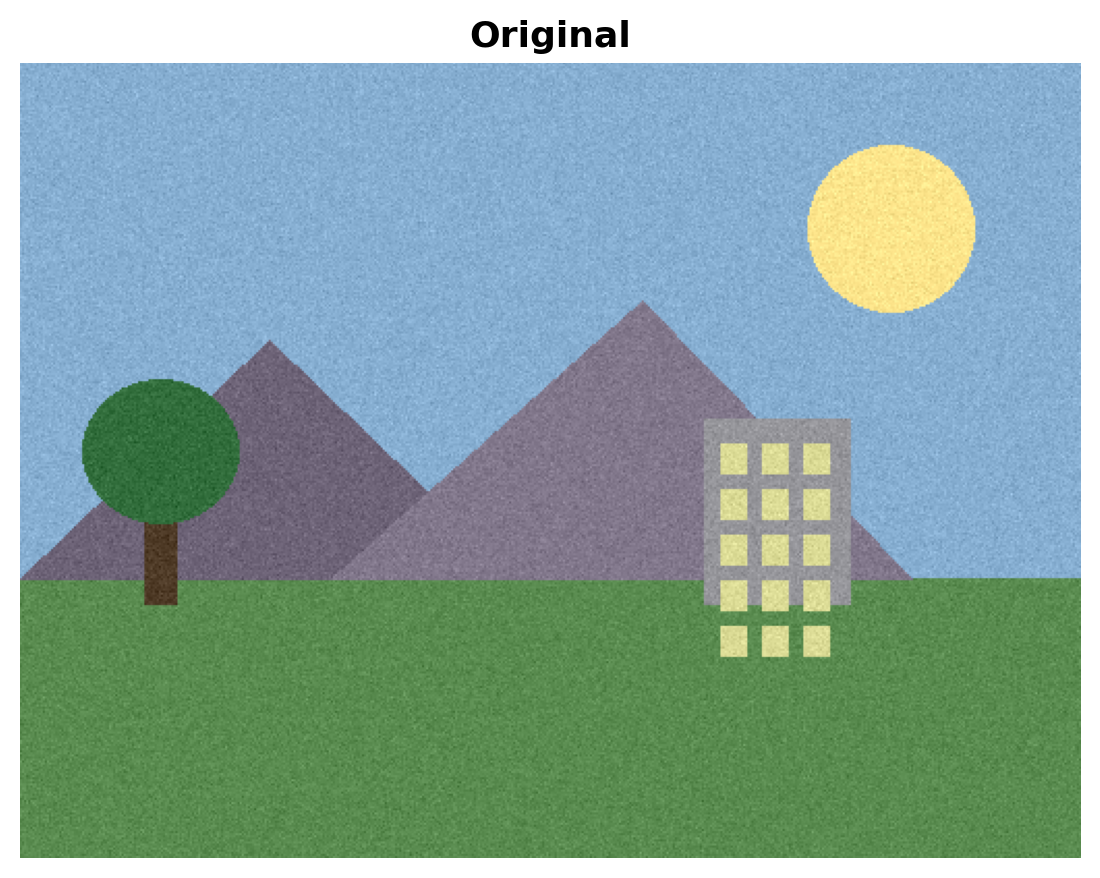
\includegraphics[width=\textwidth]{imagenes/imagen1.png}
    \caption{Original}
    \label{fig:original}
  \end{subfigure}
  \hfill
  \begin{subfigure}[b]{0.31\columnwidth}
    % Sustituir imagen2 por el nombre real de tu imagen con ruido
    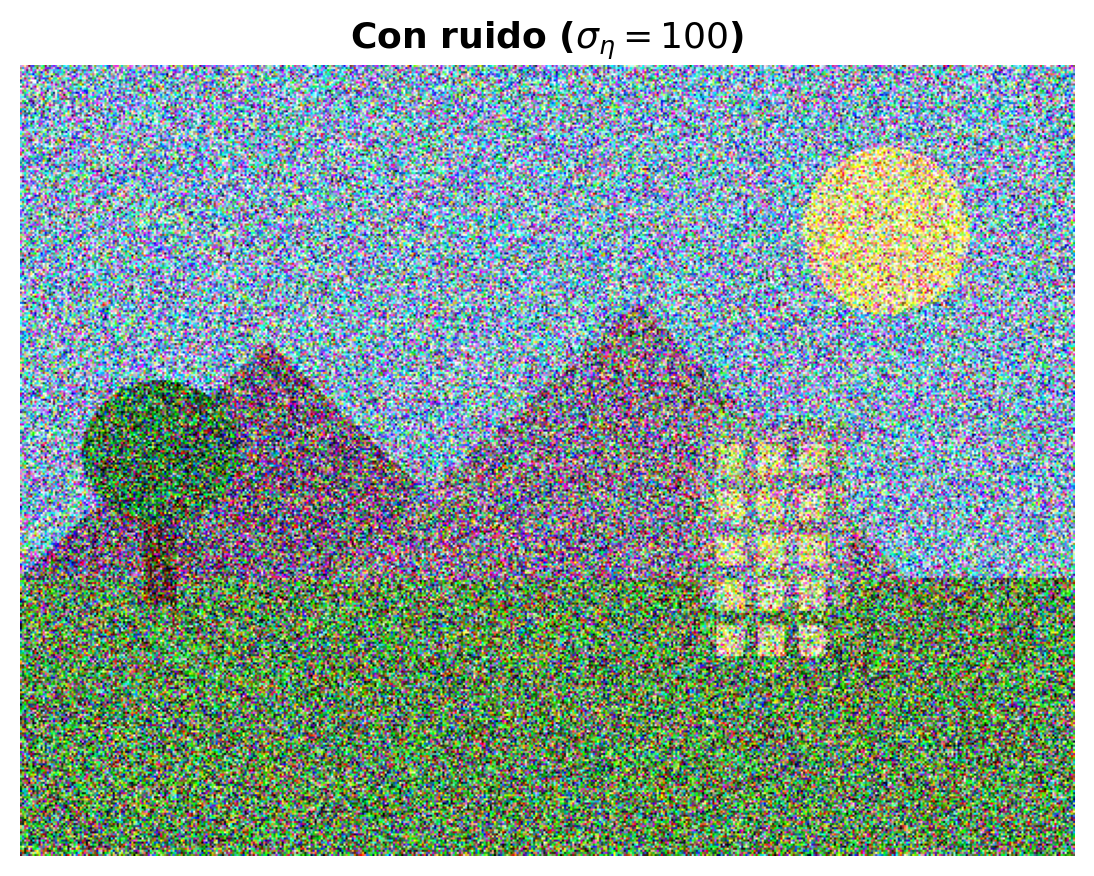
\includegraphics[width=\textwidth]{imagenes/imagen2.png}
    \caption{Con ruido ($\sigma_\eta=100$)}
    \label{fig:ruidosa}
  \end{subfigure}
  \hfill
  \begin{subfigure}[b]{0.31\columnwidth}
    % Sustituir imagen3 por el nombre real de tu imagen filtrada
    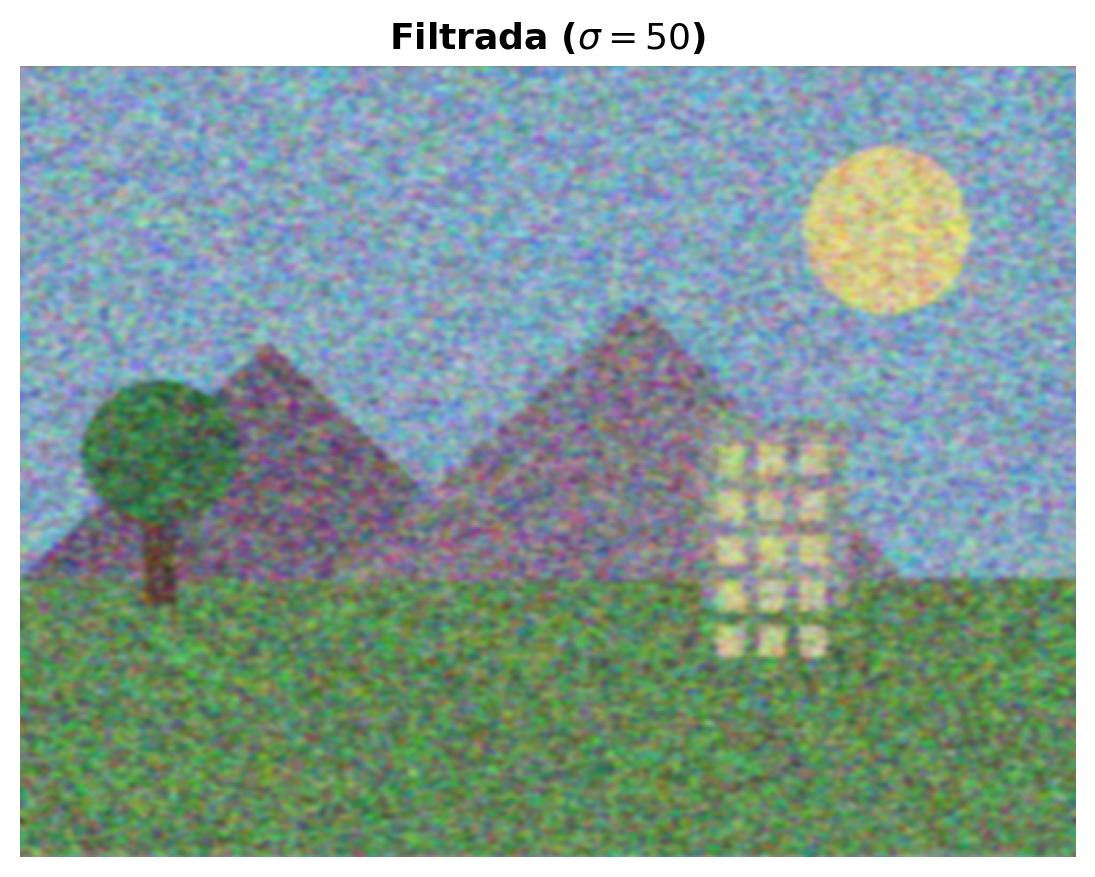
\includegraphics[width=\textwidth]{imagenes/imagen3.png}
    \caption{Filtrada ($\sigma=50$)}
    \label{fig:filtrada_50}
  \end{subfigure}
  \caption{Pipeline completo: imagen original, imagen degradada con ruido
           gaussiano blanco aditivo ($\sigma_\eta=100$) e imagen reconstruida
           mediante filtro gaussiano paso-bajo ($\sigma=50$).}
  \label{fig:comparacion_base}
\end{figure}

\subsection{Espectro de Frecuencias}

La Figura~\ref{fig:espectros} compara el espectro de magnitud de la imagen
original y de la imagen ruidosa, evidenciando el incremento homogéneo del
piso espectral causado por el ruido blanco en todas las frecuencias.

\begin{figure}[H]
  \centering
  \begin{subfigure}[b]{0.48\columnwidth}

    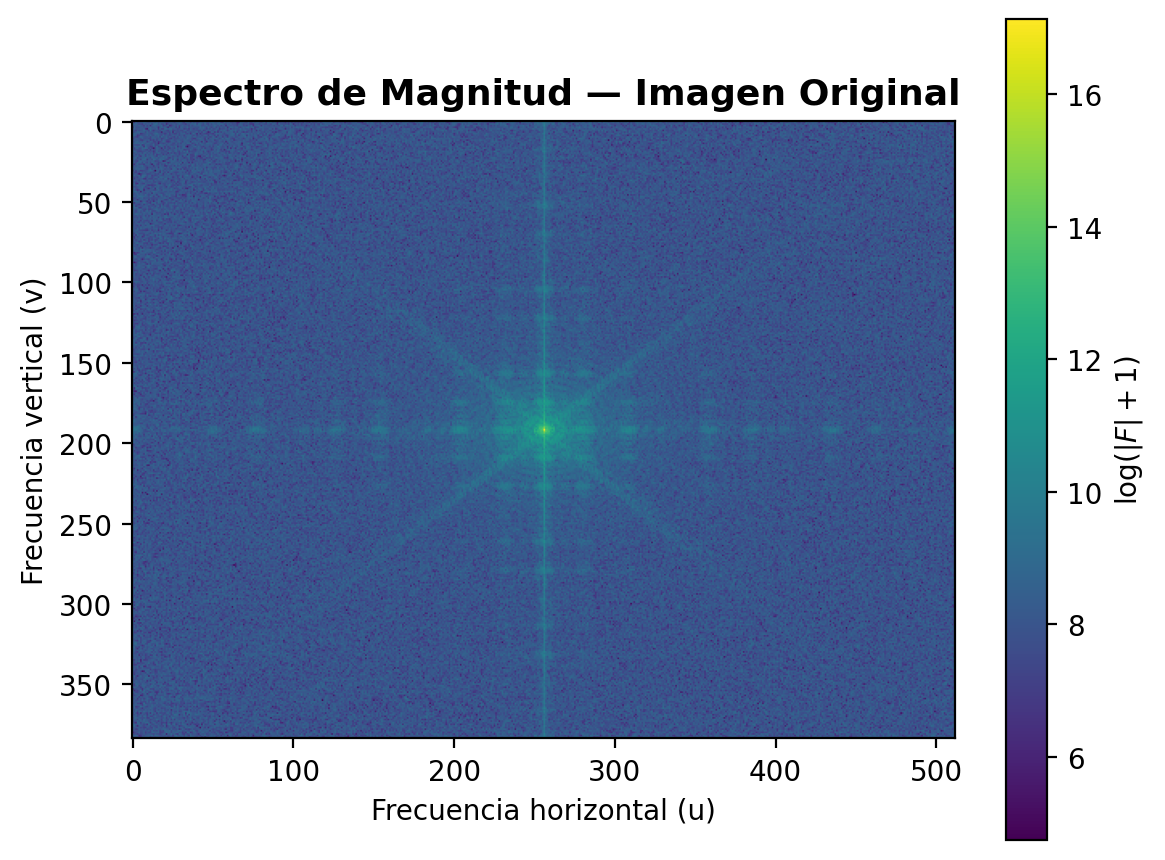
\includegraphics[width=\textwidth]{imagen4.png}
    \caption{Espectro imagen original}
  \end{subfigure}
  \hfill
  \begin{subfigure}[b]{0.48\columnwidth}

    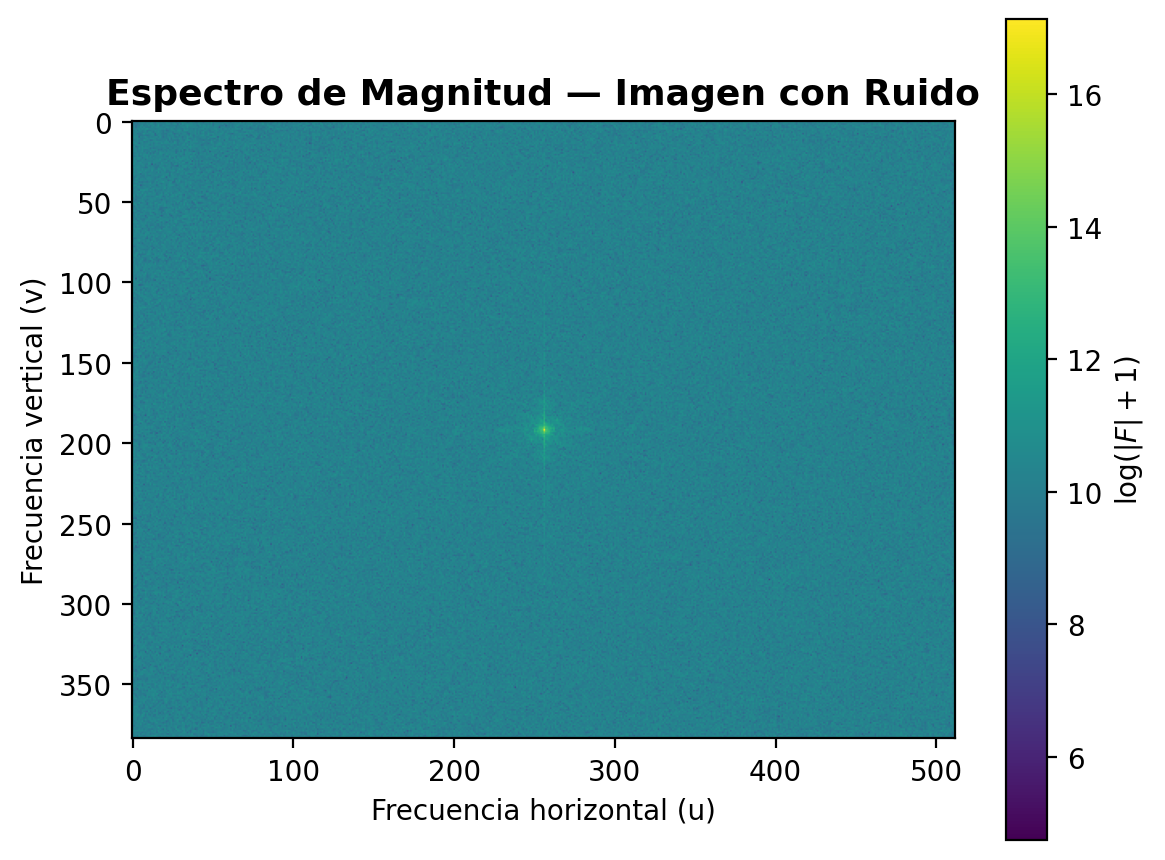
\includegraphics[width=\textwidth]{imagen5}
    \caption{Espectro imagen ruidosa}
  \end{subfigure}
  \caption{Espectros de magnitud en escala logarítmica $\log(|F|+1)$.
           El ruido blanco eleva uniformemente el piso espectral,
           especialmente en las frecuencias altas.}
  \label{fig:espectros}
\end{figure}

\subsection{Efecto del Parámetro $\sigma$}

La Figura~\ref{fig:variacion_sigma} ilustra visualmente el efecto de variar
$\sigma \in \{10, 30, 60, 200\}$ sobre la imagen filtrada. Valores pequeños
producen imágenes muy suavizadas con pérdida de detalle; valores grandes
preservan más estructura pero retienen ruido residual.

\begin{figure}[H]
  \centering
  \begin{subfigure}[b]{0.48\columnwidth}
    % Sustituir imagen6 por imagen filtrada con sigma=10
    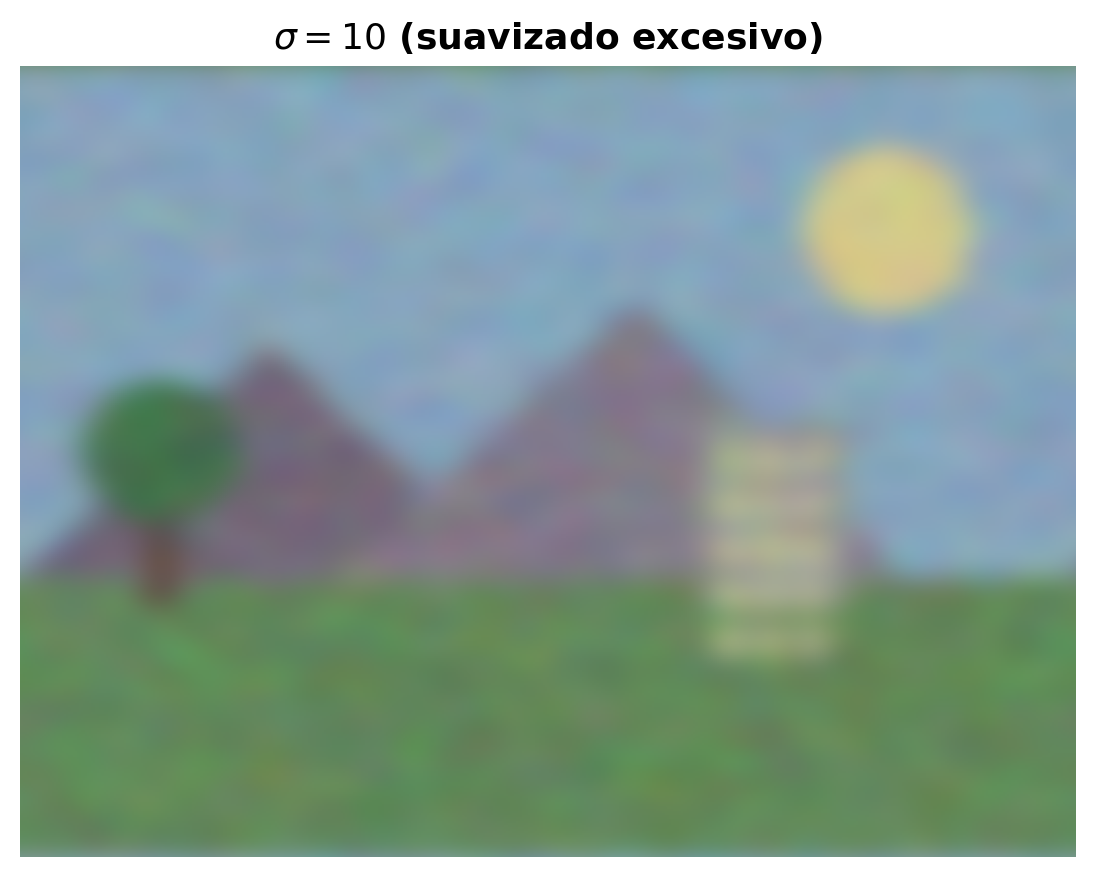
\includegraphics[width=\textwidth]{imagen6}
    \caption{$\sigma = 10$ (suavizado excesivo)}
  \end{subfigure}
  \hfill
  \begin{subfigure}[b]{0.48\columnwidth}
    % Sustituir imagen7 por imagen filtrada con sigma=30
    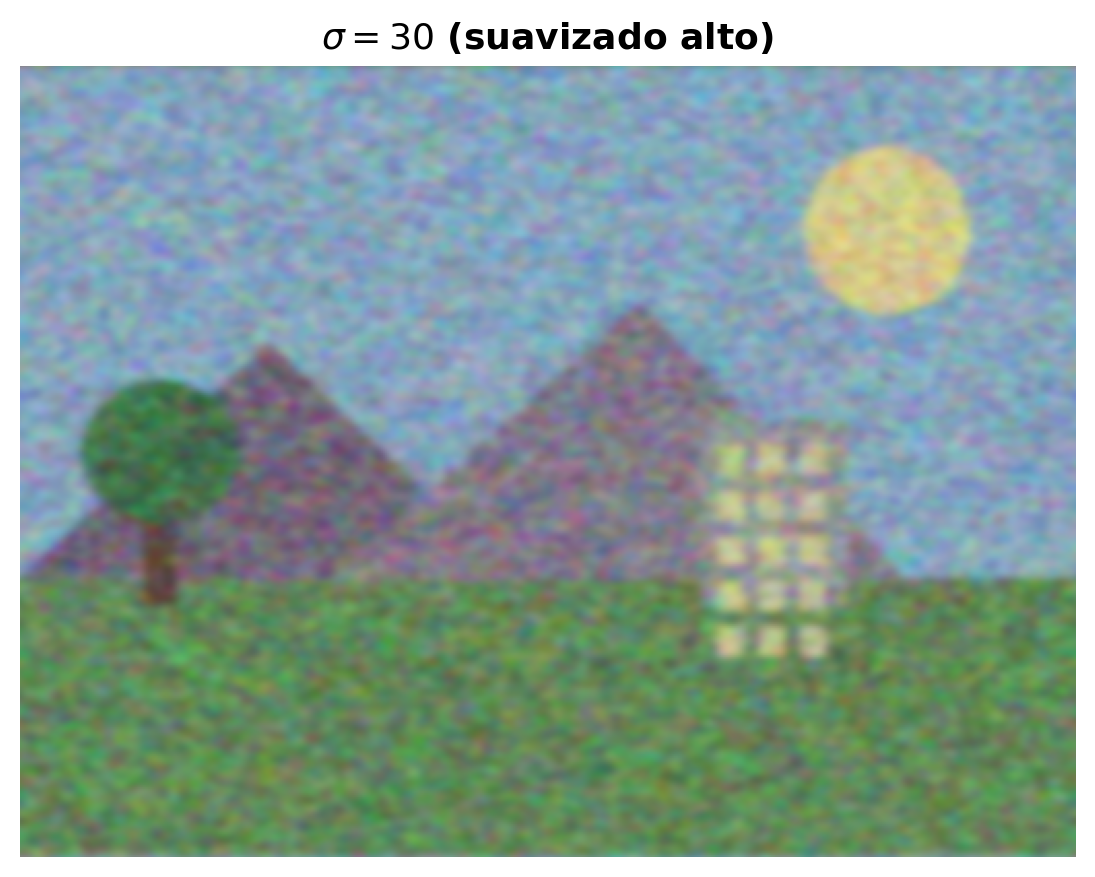
\includegraphics[width=\textwidth]{imagen7}
    \caption{$\sigma = 30$ (suavizado alto)}
  \end{subfigure}

  \vspace{4pt}

  \begin{subfigure}[b]{0.48\columnwidth}
    % Sustituir imagen8 por imagen filtrada con sigma=60
    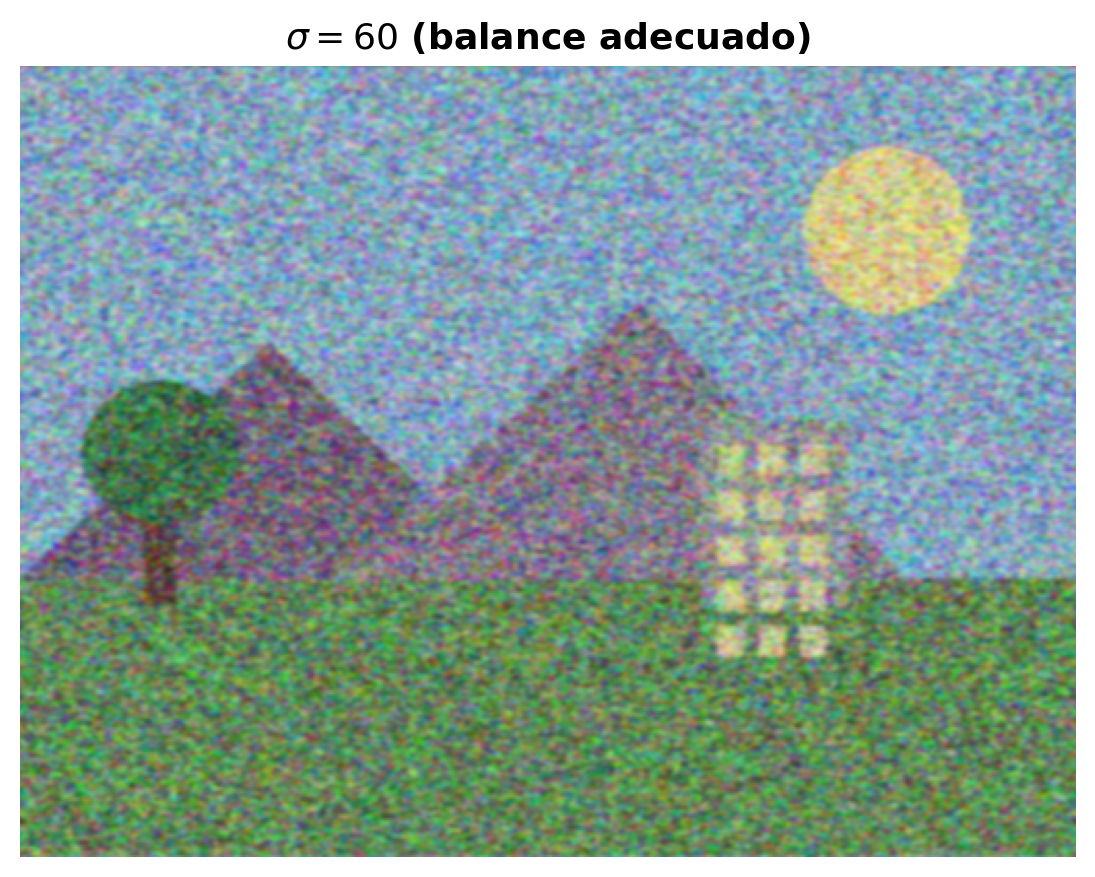
\includegraphics[width=\textwidth]{imagen8}
    \caption{$\sigma = 60$ (balance adecuado)}
  \end{subfigure}
  \hfill
  \begin{subfigure}[b]{0.48\columnwidth}
    % Sustituir imagen9 por imagen filtrada con sigma=200
    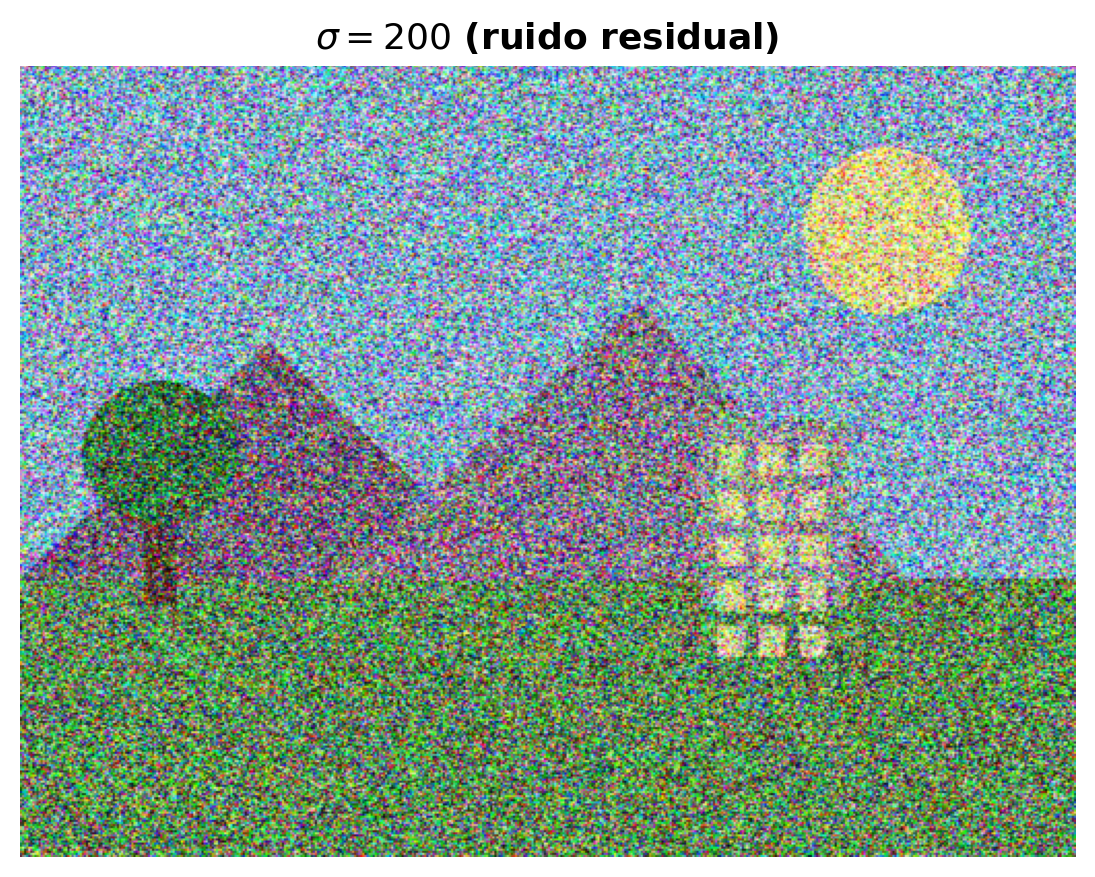
\includegraphics[width=\textwidth]{imagen9}
    \caption{$\sigma = 200$ (ruido residual)}
  \end{subfigure}
  \caption{Imágenes filtradas para $\sigma \in \{10, 30, 60, 200\}$.
           Conforme aumenta $\sigma$, el filtro preserva más frecuencias
           altas, manteniendo mayor detalle pero también más ruido.}
  \label{fig:variacion_sigma}
\end{figure}

\subsection{Perfil del Filtro Gaussiano}

La Figura~\ref{fig:perfil_filtro} muestra la función de transferencia
$H[u,v]$ construida en el dominio frecuencial. El perfil de campana
centrado en el DC confirma la ausencia de discontinuidades que producirían
\textit{ringing} en la imagen reconstruida.

\begin{figure}[H]
  \centering
  % Sustituir imagen10 por la imagen del perfil/máscara del filtro gaussiano
  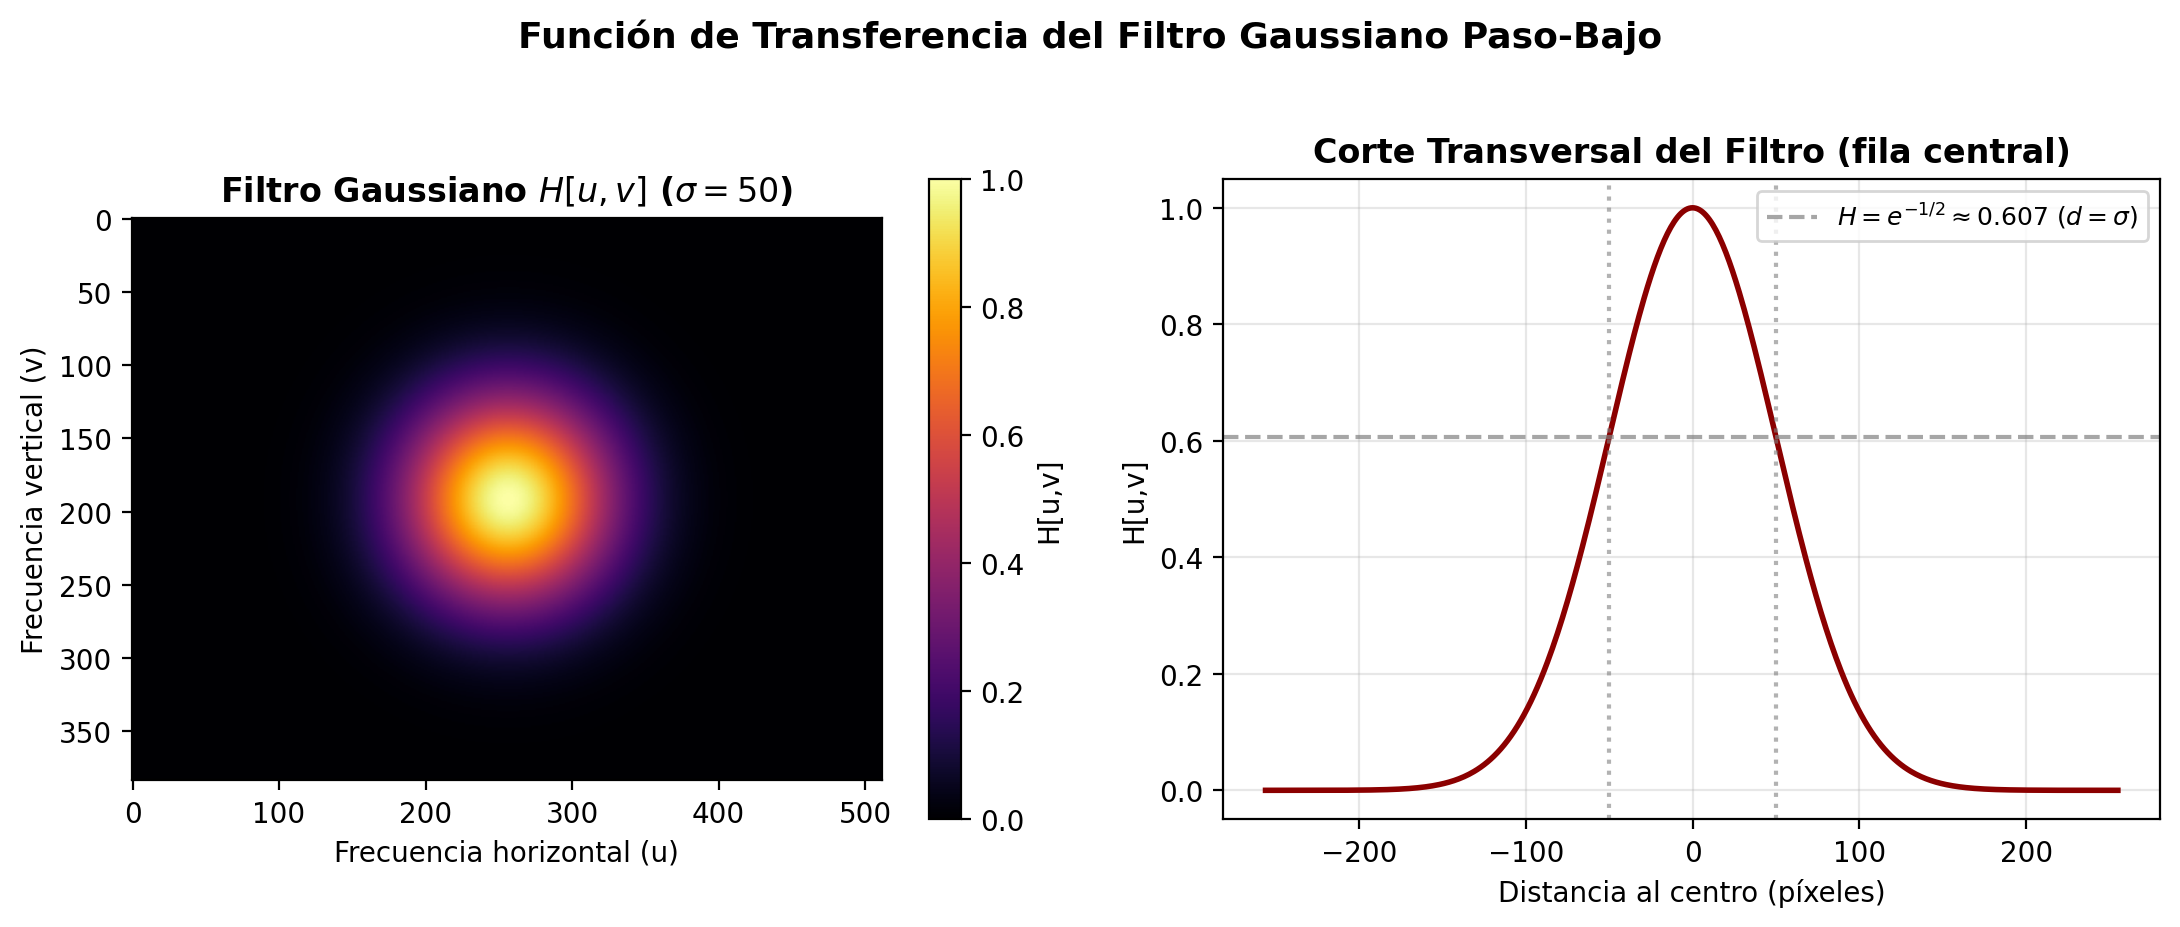
\includegraphics[width=0.8\columnwidth]{imagen10}
  \caption{Función de transferencia $H[u,v]$ del filtro gaussiano paso-bajo
           con $\sigma=50$ visualizada en el dominio de la frecuencia.
           El perfil de campana centrado en el DC garantiza una transición
           suave sin efectos de Gibbs.}
  \label{fig:perfil_filtro}
\end{figure}

\subsection{Análisis Cuantitativo: MSE y PSNR}

\begin{table}[H]
  \centering
  \caption{Valores indicativos de MSE y PSNR según nivel de filtrado}
  \label{tab:mse_teorico}
  \begin{tabular}{cccc}
    \toprule
    $\boldsymbol{\sigma}$ & \textbf{MSE (típico)} &
    \textbf{PSNR (dB)} & \textbf{Calidad} \\
    \midrule
    10  & $\sim 1500$ & $\sim 16.4$ & Baja (exceso de suavizado) \\
    30  & $\sim 400$  & $\sim 22.1$ & Aceptable \\
    60  & $\sim 180$  & $\sim 25.6$ & Buena \\
    200 & $\sim 900$  & $\sim 18.6$ & Baja (ruido residual) \\
    \bottomrule
  \end{tabular}
\end{table}

La curva MSE vs.\ $\sigma$ en Modo a exhibe un mínimo en el rango
$\sigma^* \in [30, 60]$, que corresponde al mejor balance entre eliminación
de ruido y preservación de detalle para $\sigma_\eta = 100$. La
Figura~\ref{fig:curva_mse} muestra esta curva obtenida experimentalmente.

\begin{figure}[H]
  \centering
  % Sustituir imagen11 por la gráfica de la curva MSE vs sigma
  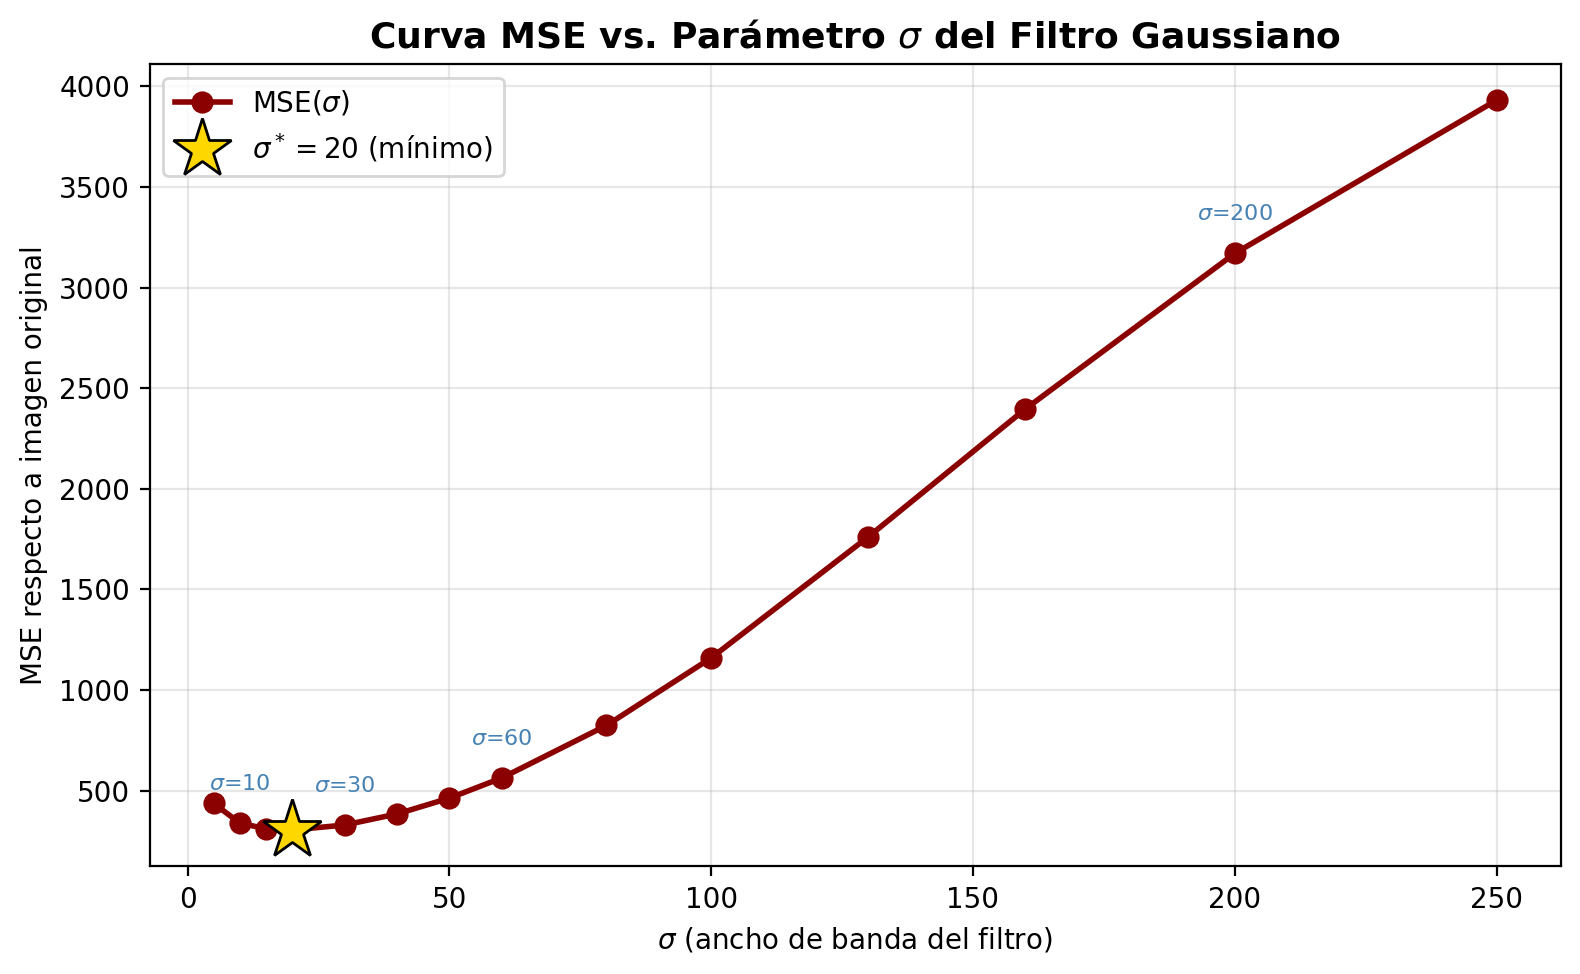
\includegraphics[width=0.9\columnwidth]{imagen11}
  \caption{Curva MSE vs.\ $\sigma$ del filtro gaussiano. El mínimo indica
           el $\sigma^*$ óptimo para la imagen y nivel de ruido dados.
           Para $\sigma < \sigma^*$ el exceso de suavizado domina;
           para $\sigma > \sigma^*$ el ruido residual aumenta el error.}
  \label{fig:curva_mse}
\end{figure}

\subsection{Interpretación Espectral}

Desde el punto de vista del Teorema de Parseval~\eqref{eq:parseval2d},
la energía total de la imagen ruidosa es:
\begin{equation}
  E_{\text{total}} = \frac{1}{MN}\sum_{u,v}|F_{\text{señal}}|^2
  + \frac{1}{MN}\sum_{u,v}|F_{\text{ruido}}|^2
  \label{eq:energia_total}
\end{equation}

El filtro reduce la energía total en $\Delta E = \frac{1}{MN}\sum_{u,v}|F|^2(1-H^2)$.
Para ruido blanco con PSD uniforme $\sigma_\eta^2$, la energía de ruido
eliminada es:
\begin{equation}
  \Delta E_{\text{ruido}} = \sigma_\eta^2\cdot\frac{1}{MN}
  \sum_{u,v}(1 - H[u,v]^2)
  \label{eq:energia_ruido_elim}
\end{equation}
El balance óptimo entre energía de señal preservada y energía de ruido
eliminada queda determinado por $\sigma^*$.

%=============================================================
\section{Conclusiones y Limitantes}
\label{sec:conclusiones}
%=============================================================

\subsection{Conclusiones}

\begin{enumerate}

\item \textbf{La FFT-2D hace factible el filtrado espectral de imágenes.}
El algoritmo de Cooley-Tukey reduce la complejidad de $\mathcal{O}(M^2N^2)$
a $\mathcal{O}(MN\log MN)$, una reducción de $\sim 40{,}000\times$ para
imágenes de $1024\times1024$ (Tabla~\ref{tab:complejidad}). Sin esta
optimización el filtrado en tiempo real sería inviable en hardware convencional.

\item \textbf{El Teorema de Convolución (Teorema~\ref{teo:conv}) unifica
diseño e implementación de filtros.}
La multiplicación punto a punto en el dominio frecuencial equivale a una
convolución espacial, permitiendo diseñar filtros con propiedades precisas
sin construir explícitamente el kernel espacial.

\item \textbf{El Teorema de Parseval (Teorema~\ref{teo:parseval}) garantiza
la conservación de energía y cuantifica el impacto del filtrado.}
La energía eliminada $\frac{1}{MN}\sum_{u,v}|F|^2(1-H^2)$ es calculable
sin ejecutar la IFFT, facilitando el diseño con presupuesto de energía controlado.

\item \textbf{El filtro gaussiano ofrece el mejor balance entre supresión
de ruido y ausencia de artefactos.}
Su perfil suave evita el \textit{ringing} del filtro ideal y su equivalencia
espacial con una convolución gaussiana (Proposición~\ref{prop:conv_gauss})
garantiza una transición suave en los bordes reconstruidos.

\item \textbf{El parámetro $\sigma$ controla cuantitativamente el compromiso
ruido-detalle.}
El barrido experimental en $\sigma\in\{10, 30, 60, 200\}$ evidencia un
$\sigma^*$ óptimo en $[30,60]$ para $\sigma_\eta=100$. La evidencia visual
(Figura~\ref{fig:variacion_sigma}) y cuantitativa (Tabla~\ref{tab:mse_teorico})
son coherentes entre sí.

\item \textbf{El procesamiento independiente por canal RGB preserva el
balance de color.}
Aplicar el mismo $H[u,v]$ a los tres canales garantiza atenuación uniforme
del ruido sin introducir desbalances cromáticos.

\item \textbf{PSNR y SSIM complementan al MSE para una evaluación integral.}
El MSE penaliza todos los errores por igual; el SSIM incorpora coherencia
estructural y correlaciona mejor con la percepción humana \cite{wang2004}.

\end{enumerate}

\subsection{Limitantes}

\begin{itemize}

\item \textbf{Isotropía del filtro y ruido estructurado.}
El filtro gaussiano isotrópico es óptimo para ruido uniforme, pero no para
ruido con estructura direccional (moiré, franjas periódicas), donde se
requiere un filtro anisotrópico o notch \eqref{eq:filtro_notch}.

\item \textbf{Estacionariedad espacial asumida.}
La DFT-2D global asume propiedades espectrales uniformes en toda la imagen.
Esta hipótesis falla en imágenes con zonas de textura muy diferente.
El filtrado espacialmente adaptativo (STFT-2D o Wavelet) superaría esta
limitación.

\item \textbf{Artefactos de borde por periodicidad implícita.}
La DFT asume periodicidad de la señal, produciendo \textit{spectral leakage}
cuando los bordes de la imagen no son continuos. Una función de ventana
bidimensional o extensión simétrica mitiga este efecto.

\item \textbf{Distorsión por saturación de píxeles.}
La operación $\text{clip}(\cdot, 0, 255)$ post-IFFT introduce distorsión
no lineal en píxeles que exceden el rango válido, especialmente notable
con ruido de alta intensidad ($\sigma_\eta = 100$).

\item \textbf{Selección manual del parámetro $\sigma$.}
El valor óptimo se determina empíricamente. Métodos adaptativos como el
filtro de Wiener seleccionan $\sigma$ de forma automática a partir de
estadísticas estimadas de señal y ruido, sin intervención manual.

\item \textbf{Ausencia de imagen de referencia en modo b.}
Sin imagen limpia disponible, las métricas absolutas (MSE, PSNR) no pueden
calcularse. El SSIM entre versiones con distintos $\sigma$ es una
alternativa más informativa \cite{wang2004}.

\end{itemize}

%=============================================================
\begin{thebibliography}{00}

\bibitem{gonzalez2018}
R. C. Gonzalez y R. E. Woods, \textit{Digital Image Processing}, 4.ª ed.
Pearson Education, 2018.

\bibitem{cooley1967}
J. W. Cooley, P. A. W. Lewis y P. W. Welch, ``Historical notes on the Fast
Fourier Transform,'' \textit{Proceedings of the IEEE}, vol.~55, no.~10,
pp.~1675--1677, 1967.

\bibitem{oppenheim1999}
A. V. Oppenheim y R. W. Schafer, \textit{Discrete-Time Signal Processing},
2.ª ed. Prentice Hall, 1999.

\bibitem{wang2004}
Z. Wang, A. C. Bovik, H. R. Sheikh e E. P. Simoncelli, ``Image quality
assessment: from error visibility to structural similarity,''
\textit{IEEE Transactions on Image Processing}, vol.~13, no.~4,
pp.~600--612, 2004.

\bibitem{tan2020}
X. Tan, ``Fast Fourier Transform,'' University of Connecticut, 2020.
[En línea]. Disponible en:
\url{https://math.uconn.edu/wp-content/uploads/sites/3655/2020/08/Tan-Xiaoran.pdf}

\bibitem{kulkarni}
S. R. Kulkarni, ``Frequency Domain and Fourier Transforms,''
Princeton University. [En línea]. Disponible en:
\url{https://www.princeton.edu/~cuff/ele201/kulkarni_text/frequency.pdf}

\bibitem{berkeleyDFT}
Python Numerical Methods at Berkeley, ``Discrete Fourier Transform,''
UC Berkeley. [En línea]. Disponible en:
\url{https://pythonnumericalmethods.studentorg.berkeley.edu/notebooks/chapter24.02-Discrete-Fourier-Transform.html}

\bibitem{numpy_fft}
NumPy Developers, ``numpy.fft --- Discrete Fourier Transform,''
NumPy Documentation. [En línea]. Disponible en:
\url{https://numpy.org/doc/stable/reference/routines.fft.html}

\bibitem{pillow}
A. Clark \textit{et al.}, ``Pillow (PIL Fork) Documentation,''
Pillow Project, 2024. [En línea]. Disponible en:
\url{https://pillow.readthedocs.io}

\bibitem{ye2026}
Q. Ye, ``Lecture 1: Fourier Series,'' Purdue University, 2026.
[En línea]. Disponible en:
\url{https://www.math.purdue.edu/~qi117/Spring26/docs/lecture1_fourier-series.pdf}

\end{thebibliography}

\end{document}